% !TEX encoding = UTF-8 Unicode
% -*- coding: UTF-8; -*-
% vim: set fenc=utf-8

\section{Algoritmy používané pro kolaborativní editaci textů}\label{sec:algoritmyProKolaborativníEditaci}

Synchronizace dvou a více kopií stejného dokumentu ve skutečném čase je komplexní problém.
V této části popisuji dva nejznámější a nejrozšířenější algoritmy pro synchronizaci textu mezi více klienty při použití architektury klient-server~\cite{algoritmy:first}.

\subsection{Druhy algoritmů}

Existují tři nejčastější přístupy k problému synchronizace, metoda zamykání (nebo také vlastnictví), předávání událost a třísměrné sloučení.

Metoda \textbf{zamykaní} je nejjednodušší technika.
Ve své nejčastější formě může dokument v jednu chvíli editovat pouze jeden uživatel a to ten který si dokument uzamkl.
Ostatní uživatele mohou dokument pouze číst.
Provádět změny mohou pouze po uvolnění zámku, stažení nové verze dokumentu a přivlastnění jeho zámku.

Některé vylepšené algoritmy na základě uzamykání se pokouše automaticky uzamykat pouze upravované části dokumentu.
To však zamezuje úzké spolupráci více uživatel nad dokumentem, protože každý může pracovat pouze na své části dokumentu.

Metoda \textbf{předávání událost} spočívá v myšlence zachycení vše změn provedených nad dokumentem a jejich provedení nad všemi kopiemi zároveň.
Hlavní představitelem tohoto přístupu je právě operační transformace o které píší níže v~\ref{subsec:operacniTransformace}.

Hlavním problémem tohoto přístupu je zachycení všech změn dokumentu, které mohou být triviální jako je například napsání znaku, ale také například vložení obrázku, přetažení velkého množství textu, automatická oprava překlepů a mnoho dalších.
Přístup předávání událostí není přirozeně konvergentní.
Každá změna, která není správně zachycena (nebo ztracena při cestě po síti), vytváří novou verzi dokumentu, kterou již není možné správně obnovit.

Poslední častou metodou je takzvané \textbf{třísměrné sloučení}.
Uživatel odešle svůj změněný dokument na server, který provede sloučení s aktuální verzí na serveru a uživateli pošle novou sloučenou verzi zpět.
Pokud uživatel provedl v době synchronizace v dokumentu změny novou verzi ignoruje a musí to zkusit později.

Jedná se poloduplexní systém, dokud uživatel píše nedostává žádné aktualizace o dokumentu a ve chvíli co přestane psát zobrazí se všechny změny od ostatních uživatel nebo vyskočí hláška o nastalé kolizi (to samozřejmě záleží na použitém slučovacím algoritmu).~\cite{ds:neil_paper, ds_neil_video}

\enquote{Tento system lze přirovnat k automobilu s čelním sklem, které se stane během jízdy neprůhledné.
Podívej se na cestu, pak jeď chvilku poslepu, pak zastav a podívej se znovu.
Kdyby všichni řídili stejný druh \enquote{dívej se a nebo jeď} automobilů, těžké nehody by byly velmi časté.}~\cite{ds:neil_paper} přeložil Jiří Šimeček.

Příkladem systému, který používá třísměrné sloučené je například SVN\footnote{Apache Subversion - systém pro správu zdrojových kódů}.

\subsection{Diferenciální synchronizace}\label{subsec:diferencialniSynchronizace}

\gls{DS} je algoritmus, který vymyslel Neil Fraser a lze považovat za zástupce třísměrného sloučení.
\gls{DS} řeší problém s průběžnou synchronizací, kterým trpí klasický model třísměrného sloučení, a to použitím stínových kopií a diff-patch algoritmu nejen na serveru, ale i u každé kopii dokumentu.

Na obrázek číslo~\ref{fig:DS_diagram} je vidět zjednodušený vývojový diagram \gls{DS} algoritmu.
Diagram předpokládá dva dokumenty (pojmenované server text a klient text), které jsou umístěné na stejném počítači a tedy nepočítá se síťovou dobou odezvy.

\begin{figure}[ht]
    \centering
    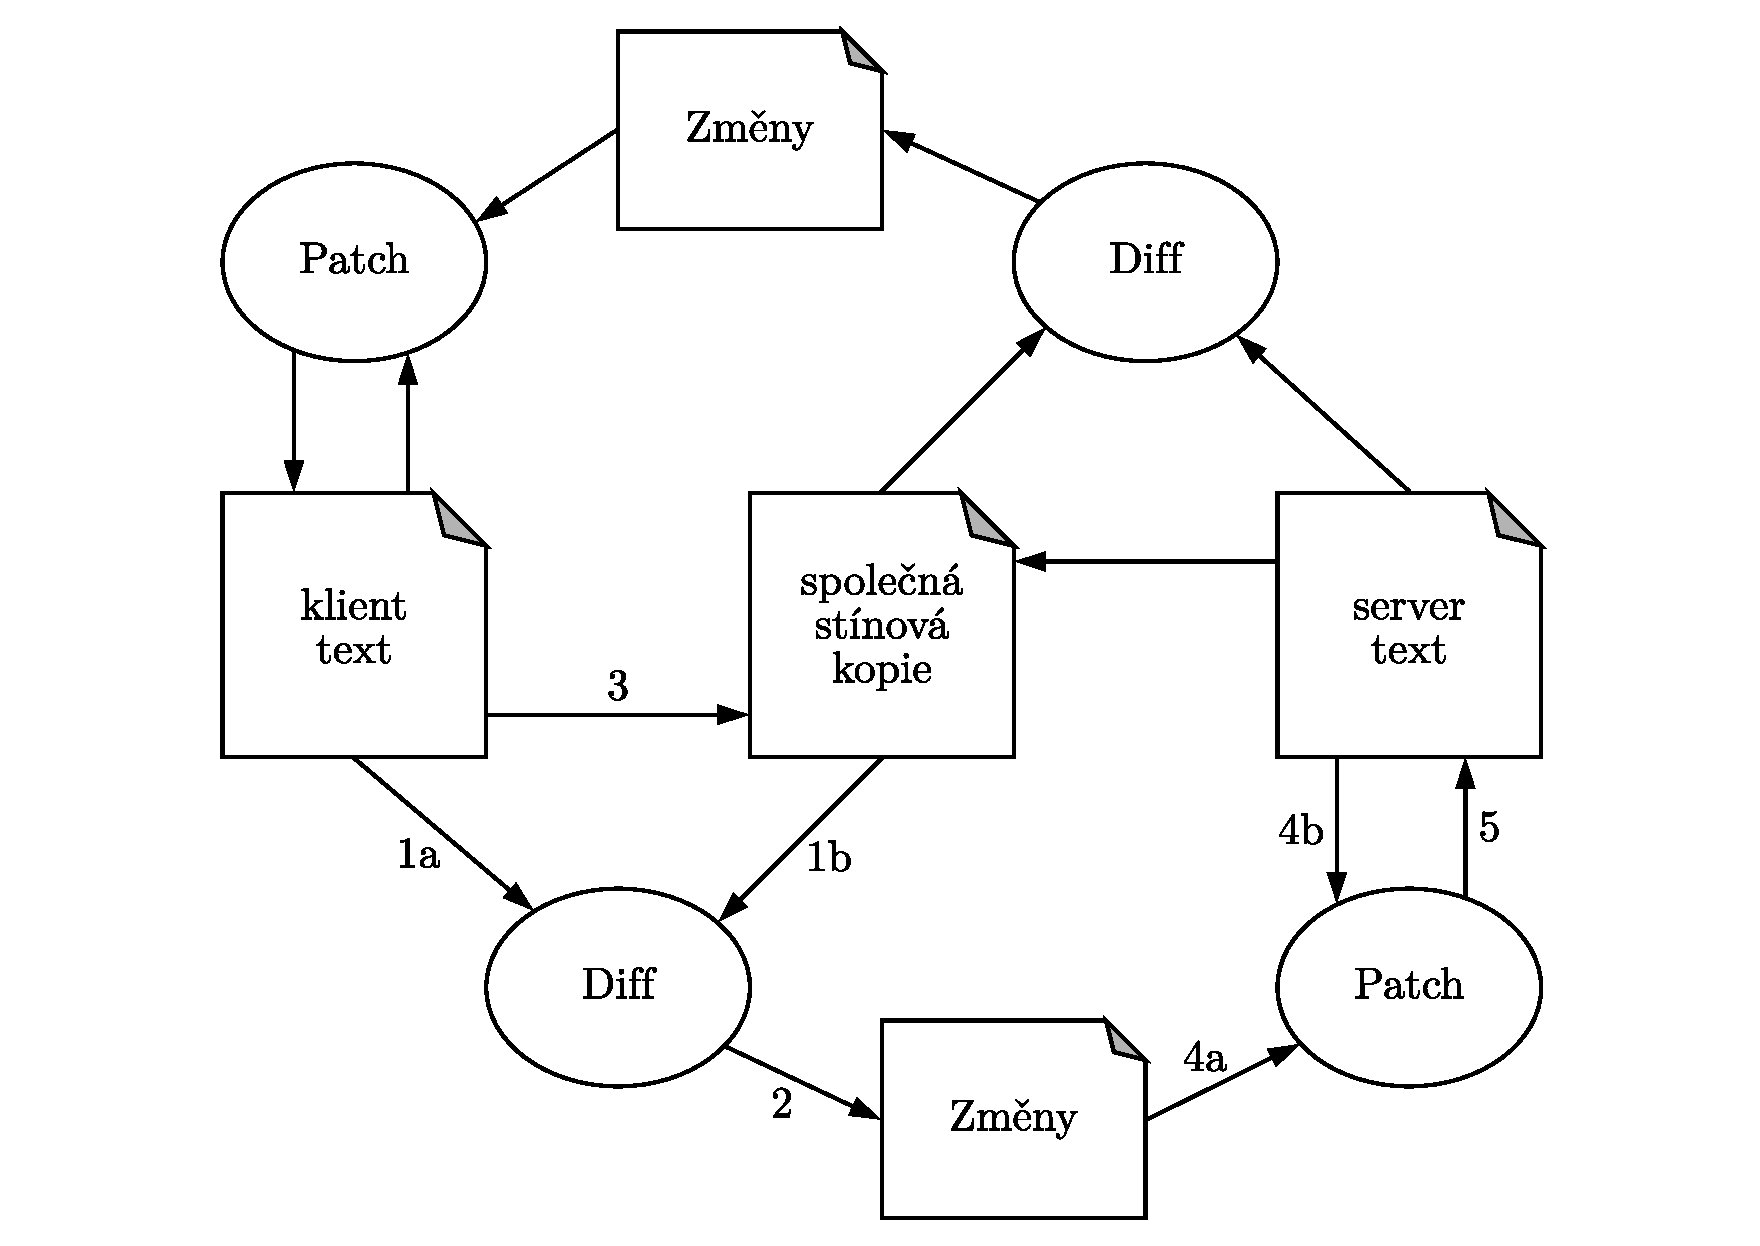
\includegraphics[width=\textwidth]{partials/analyza/DS_diagram.pdf}
    \caption{Diferenciální synchronizace vývojový diagram~\cite{ds:neil_paper}}\label{fig:DS_diagram}
\end{figure}

Na začátku jsou všechny dokumenty stejné (klient text, server text i společná stínová kopie).
Klient text i server text mohou být libovolně upraveny a naším cílem je udržet oba dokumenty neustále co nejvíce podobné.

Algoritmus pokračuje následujícími kroky (viz čísla u jednotlivých přechodů diagramu~\ref{fig:DS_diagram}):
\begin{enumerate}
    \item klient text je porovnán oproti společní stínové kopii,
    \item výsledkem porovnání je seznam změn, které byly provedeny na klient text kopii dokumentu,
    \item klient text je překopírován přes společnou stínovou kopii,
    \item seznam změn je aplikován na server text (za použití best-effort math algoritmu),\label{krok:aplikace}
    \item server text je přepsán výsledkem aplikace změn.\label{krok:prepsani}
\end{enumerate}

Důležité je, že pro správné fungování musí být kroky~\ref{krok:aplikace} a~\ref{krok:prepsani} atomické, tedy nesmí se stát, že by se server text v tuto chvíli změnil.

Algoritmus předpokládá použití libovolného diff-patch algoritmu, který umožňuje aplikovat změny i na dokument, který se změnil.
Lze například použít diff-patch-match\footnote{https://github.com/google/diff-match-patch} algoritmus od společnosti Google.
Ten implementuje diff algoritmus od Eugene W. Myers, který je považování za nejlepší obecně použitelný diff algoritmus~\cite{ds:myers_diff}.~\cite{ds:neil_paper, ds:neil_video}

\subsection{Operační transformace}\label{subsec:operacniTransformace}

\gls{OP} je algoritmus, který se poprvé objevil v \ldots

